\chapter{Results}
\label{chap:results}

\section{Simple Approach to Data Set Acquisition}
The biggest acheivement of this \master is to enable
Following is the complete list of steps required to start the \sr and record video.
\begin{enumerate}
    \item Connect the battery to the \jx.
    \item Enable mobile hotspot on your phone with name and password set to\textit{sensorrig}.
    \item Wait for the \sr to connect and find its IP address under hotspot settings.
    \item Go to \textit{http://<ip-address>:8080} in a web browser.
    \item Start the recording in the \textit{Run} tab.
    \item Start the \gls{ptp} deamons in the \gls{ptp} tab.
    \item Collect your dataset and monitor the video in the \textit{Video} tab.
\end{enumerate}


\section{Stereo Polarization Data}
The \sr is capable of reliably capturing 10-bit video at 16fps.
A simple visualization toolkit was developed that uses the Equation \todo
to calculate \gls{dolp} and \gls{aolp} and visualize this as hue and value in the \gls{hsv} color space.
Figure shows one of the captured images with this visualization applied below.
The image clarely shows ghe potential benefit of polarization imaging in maritime environments.
Five reagions of interest are marked in the image and discussed in the following sections.

\begin{figure}[H]
    \centering
    \subcaptionbox{Avraged image. Simliar to "normal" camera. \label{fig:normal_img_1536}}{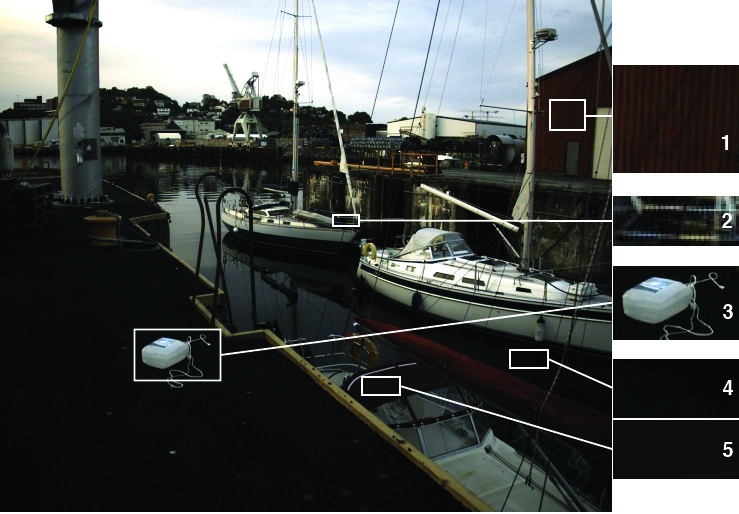
\includegraphics[width=\textwidth]{figures/pictures/result_rgb-80.jpg}}
    \subcaptionbox{\gls{aolp} and \gls{dolp} visualized as hue and value. \label{fig:pol_img_1536}}{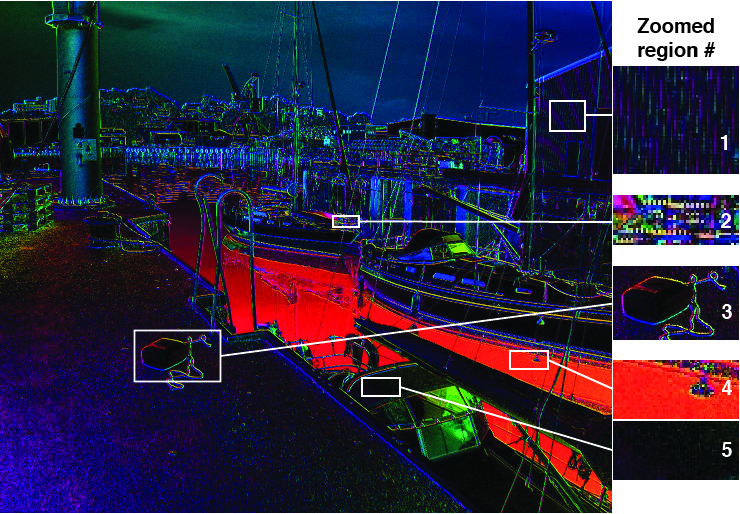
\includegraphics[width=\textwidth]{figures/pictures/result_pol-80.jpg}}
    \caption{Right image \#1536 with, zoomed in regions of interest.}
    \label{fig:picture_1536}
\end{figure}

\subsection{Region 3: Artificial Polarization fom Gradients}
\label{sec:artifical_polarization}
Region 3 shows what is believed to be artificial polarization.
As the four angles of polarization are spatially separated in the \gls{pfa}, high image gradients is believed to cause the polarization angle to be estimated incorrectly.

Papers on polarization estimation techniques have been written for both monocrome and color polariztion cameras  \cite{mihoubiSurveyDemosaickingMethods2018} \cite{spoteJointDemosaicingColour2021}, but
none of these methods were compatible with the current setup, but they could be used as inspiration for future work.
Section \ref{sec:better_analysation_tools} discusses how better analysation tools can be implemented in future works.

\subsection{Region 1: Aliasing}
As four pixels are used to form each \gls{pg}, the \gls{cg} are more spacially separated than in a normal camera.
This means that the effects such as aliasing are expected to be more pronounced.
This is seen in region 1 in Figure \ref{fig:picture_1536} where the aliasing is more pronounced than in the other regions.
The polarization of this area shows that we also have aliasing efects in the polarization domain.
It is believed that this caused by the artificial polarization discussed in Section \ref{sec:artifical_polarization}.

\subsection{Region 2: Dithering}
Similarly to aliasing, we also observe dithering in high frequency areas.
This is seen in region 2 in Figure \ref{fig:normal_img_1536} and is further exagerated in the polarization image.
We also see some color artifacts in the regular image as what is believed to be a white bar is firs slightly blue then slightly red.
This suggests that there is room for improvement in the debayering algorithm.

\subsection{Region 4 and 5: Polarization Reveals Water}
Ths big advantage of polarization imageing in maritime environments is that water reflections are polarized.
This makes it almost trivial to detect water in the image as seen by de difference in polarization between region 4 and 5 in Figure \ref{fig:pol_img_1536}.
This effect is however weaker further back where the angle of incidense is further away from the Brewster's angle.


\subsection{10 Bit Images}
Another noteworthy benefit of the final setup is that we get images with 10 bit depth.
This give the images higher dynamic range as the pixel values are more nuanced.
A visualization of this is is shown in Figure \ref{fig:gained_image} where digital gain is applied to the image in Figure \ref{fig:normal_img_1536}, revealing that the darker regions do contain a lot of information.
This probably contributes to why polarization information can be extracted from region 4 in Figure \ref{fig:picture_1536}.

\begin{figure}[H]
    \centering
    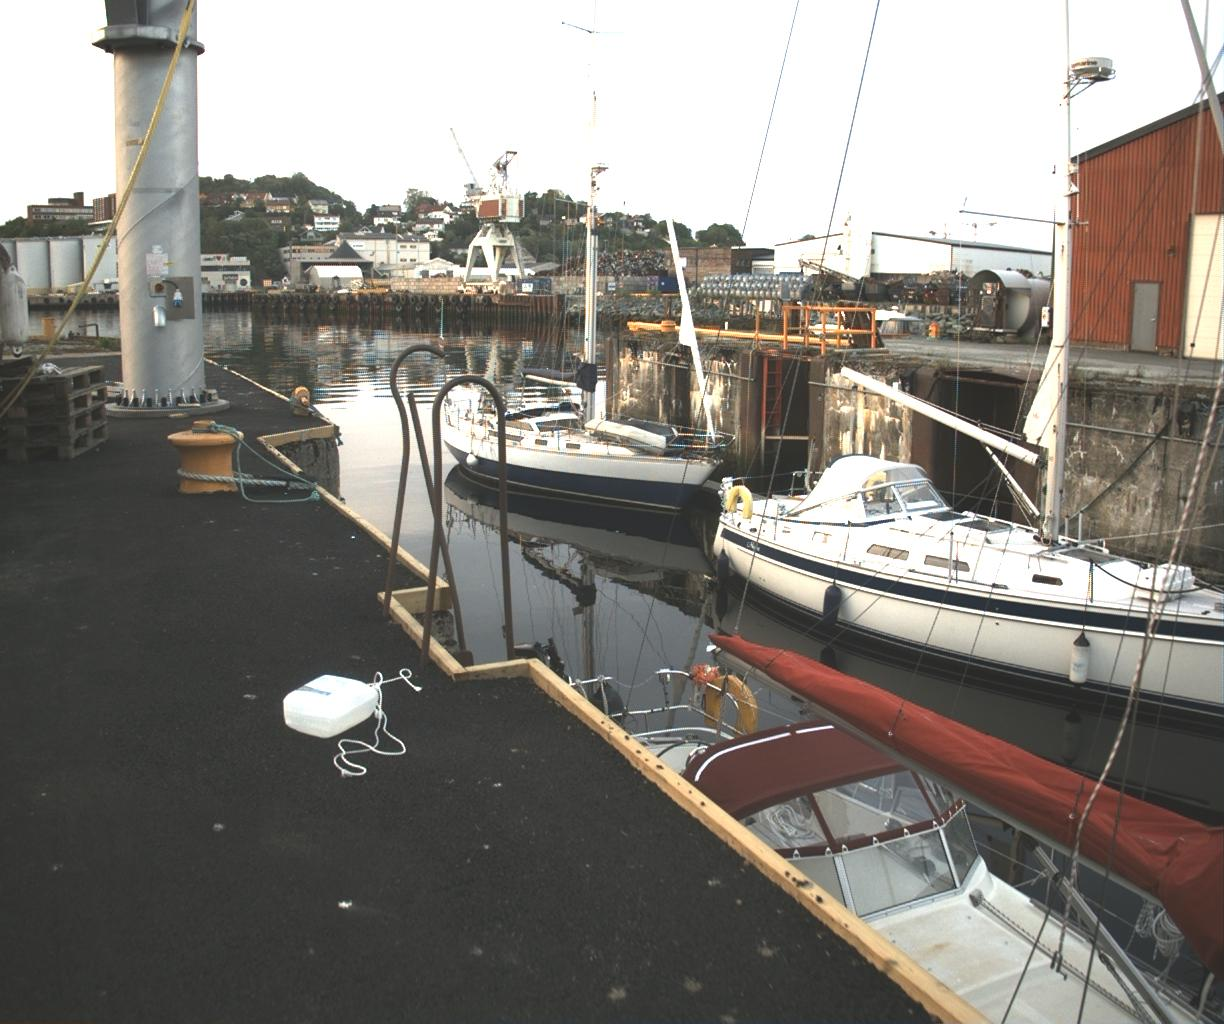
\includegraphics[width=.8\textwidth]{figures/pictures/gained_right_96.jpeg}
    \caption{Image showing how dark areas contain a lot of information thanks to 10-bit depth. The image is the same as in Figure \ref{fig:normal_img_1536}, but with digitally increased brightnes.}
    \label{fig:gained_image}
\end{figure}

\begin{figure}[H]
    \centering
    \subcaptionbox{Mean image.}{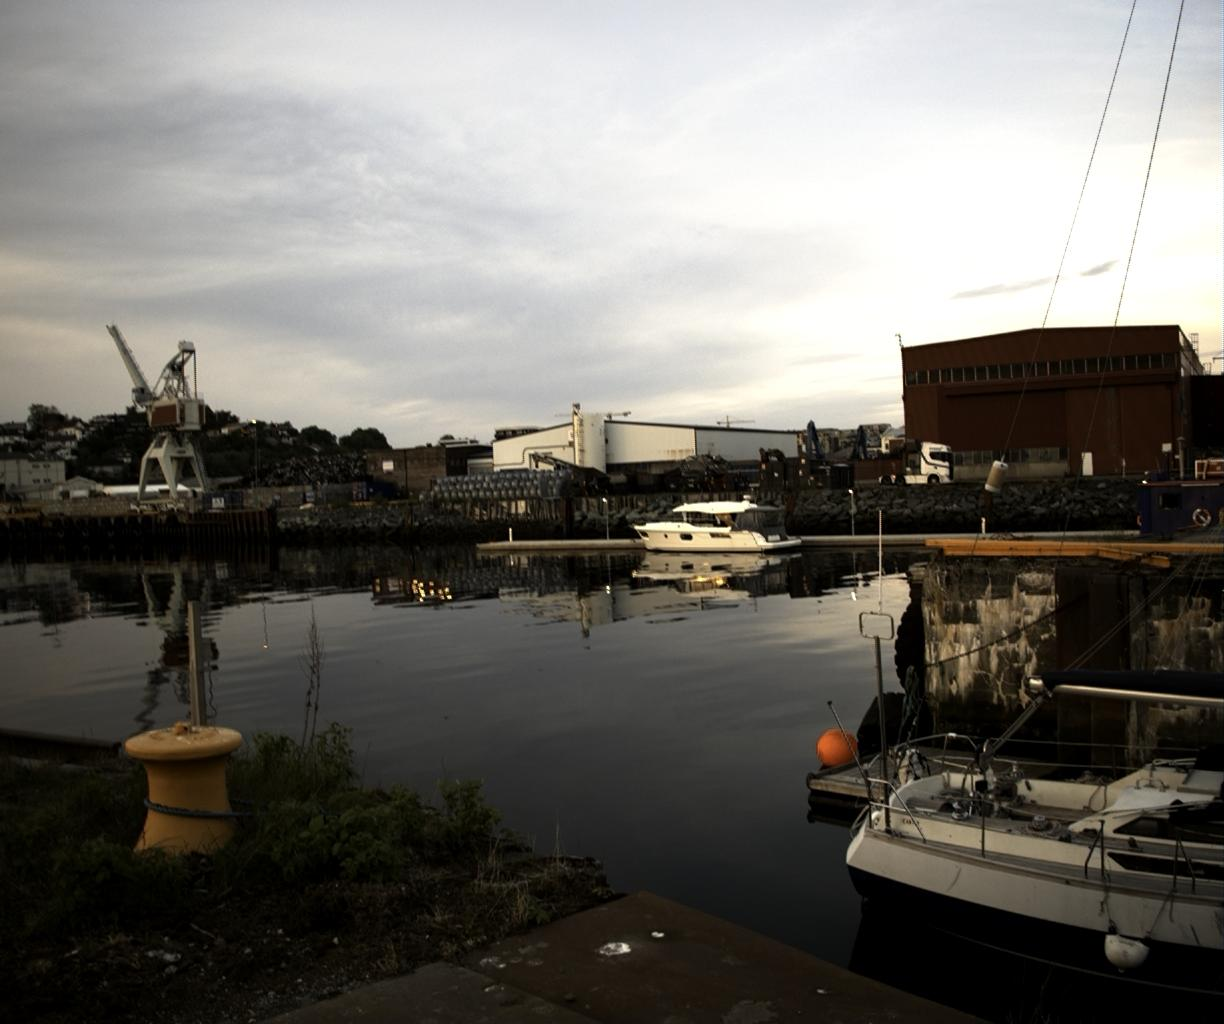
\includegraphics[width=.9\textwidth]{figures/pictures/regular_left_124.jpeg}}
    \subcaptionbox{HSV visualization.}{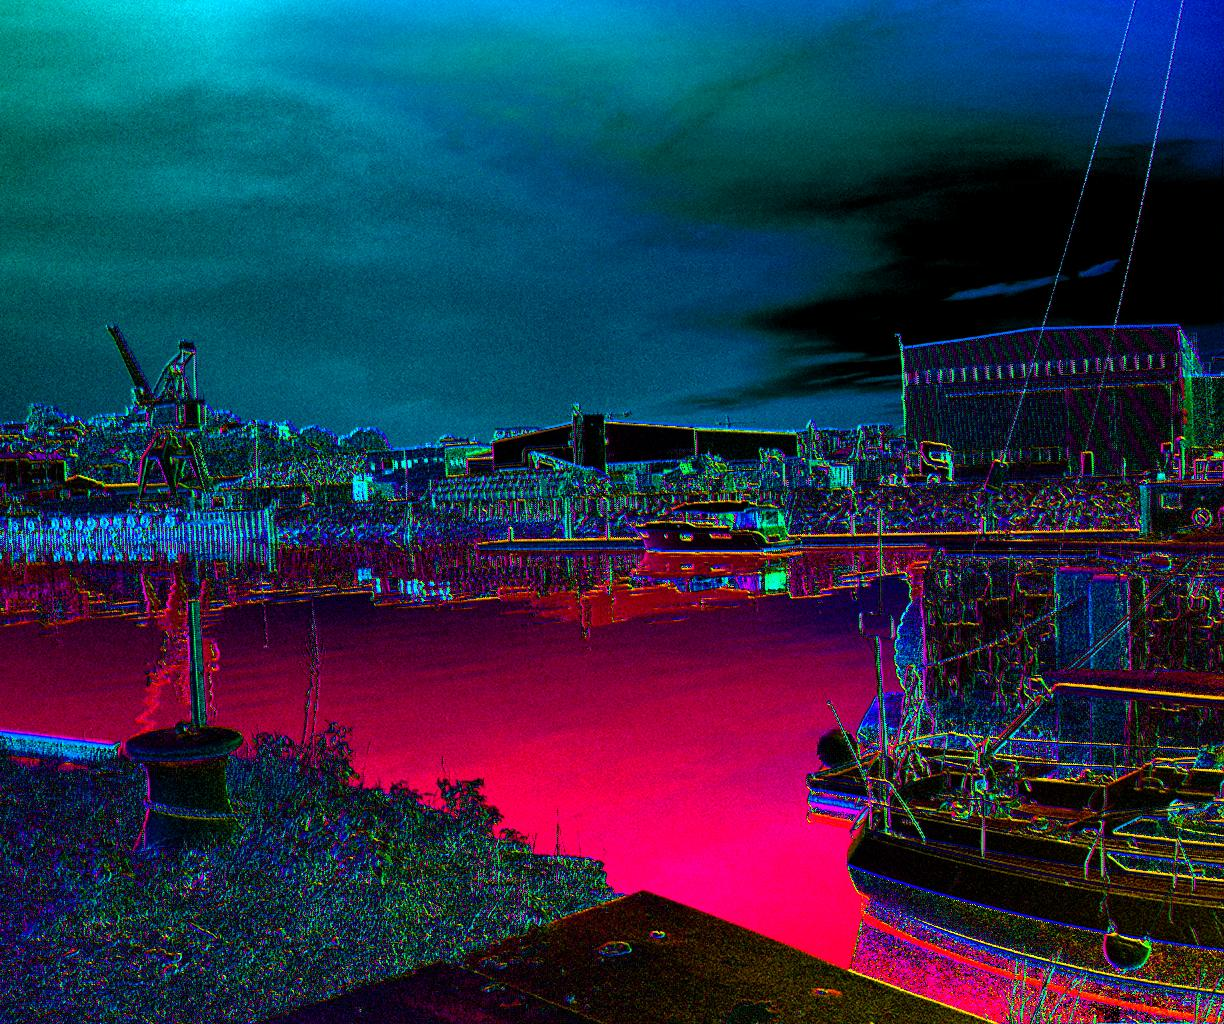
\includegraphics[width=.9\textwidth]{figures/pictures/aolp_left_124.jpeg}}
    \caption{Left image \#1984}
\end{figure}
\begin{figure}[H]
    \centering
    \subcaptionbox{Mean image.}{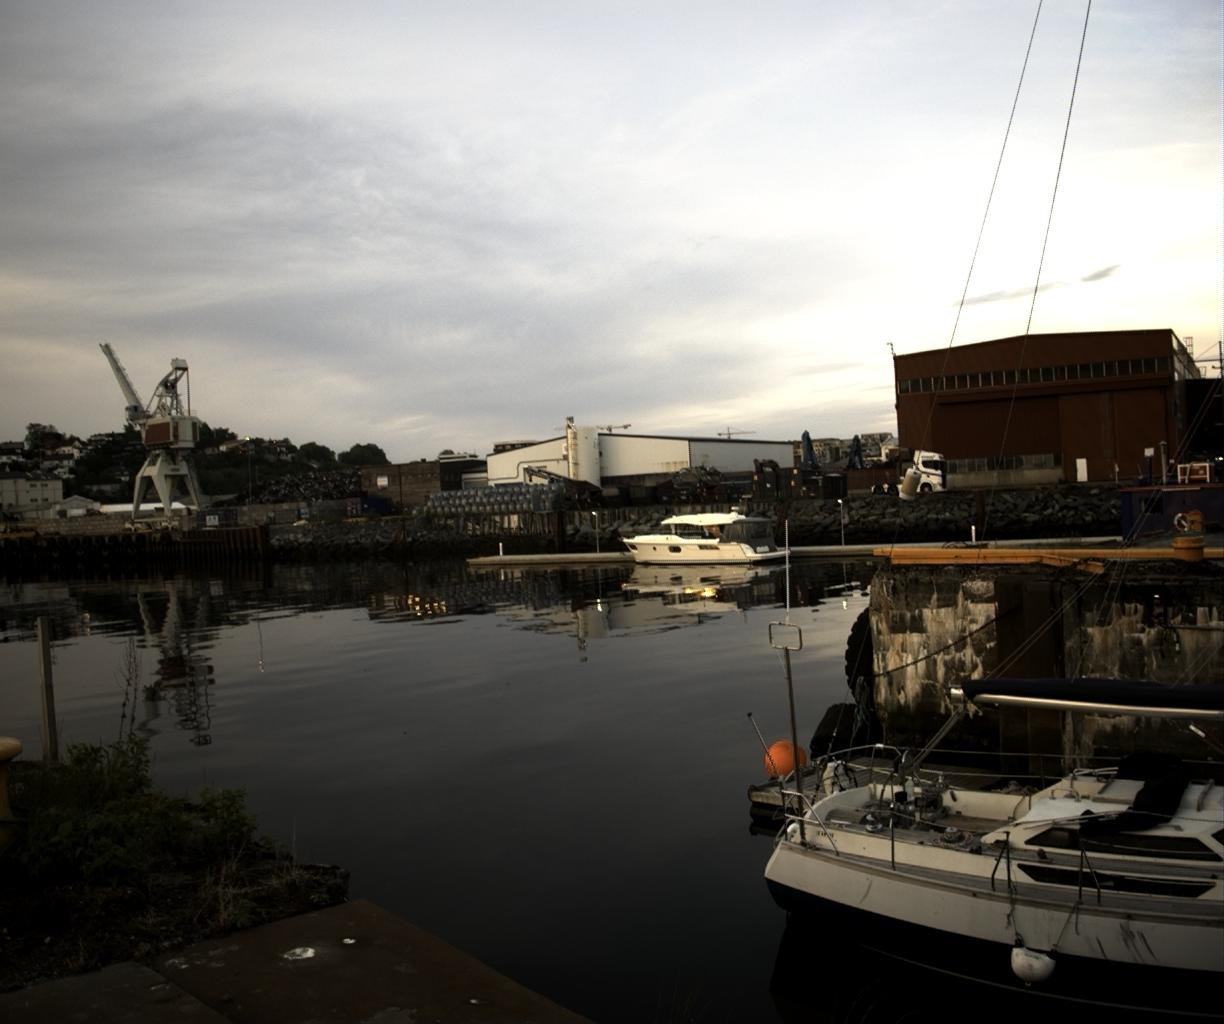
\includegraphics[width=.9\textwidth]{figures/pictures/regular_right_124.jpeg}}
    \subcaptionbox{HSV visualization.}{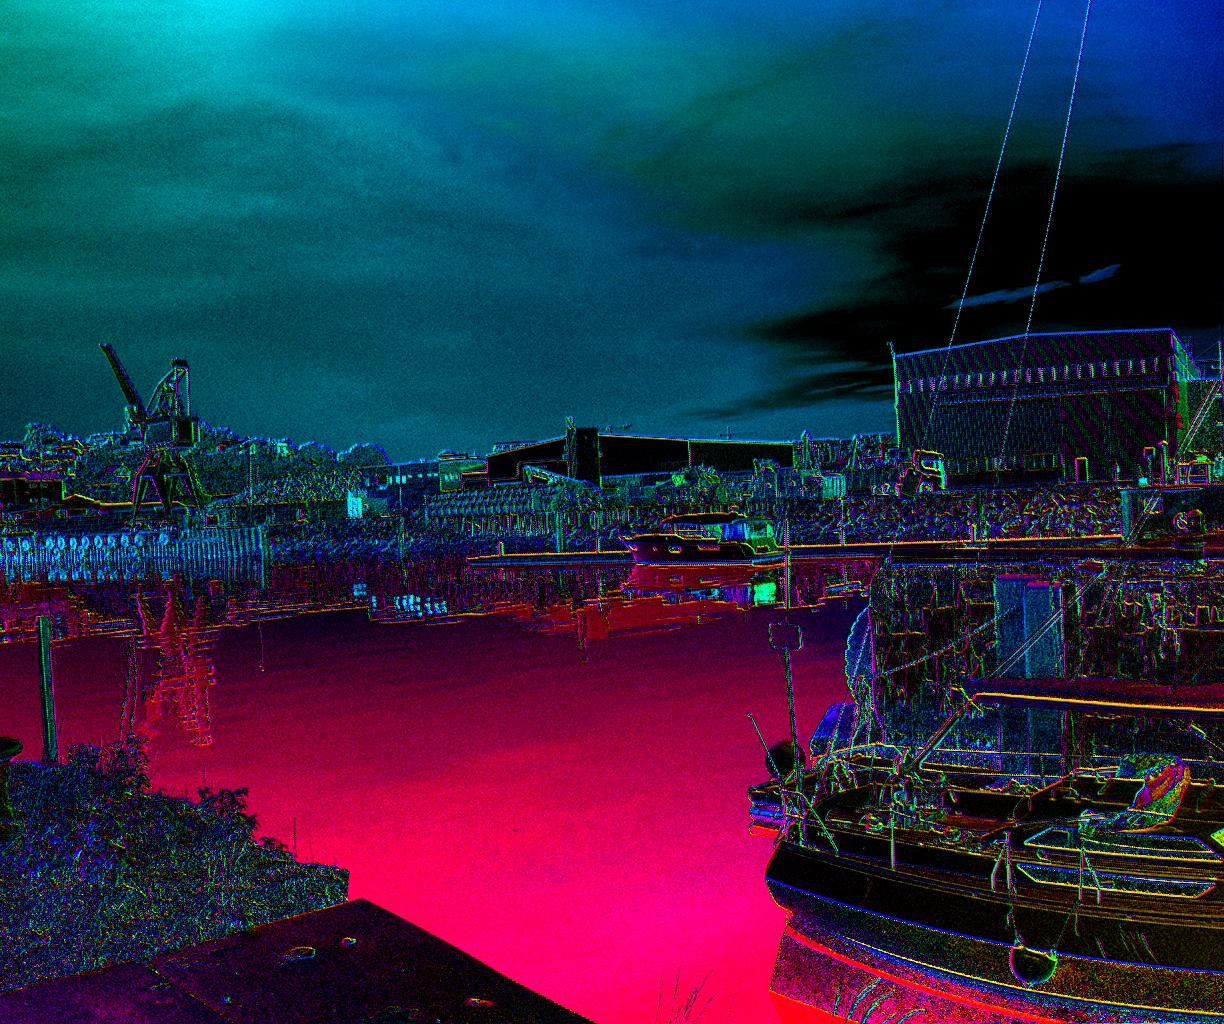
\includegraphics[width=.9\textwidth]{figures/pictures/aolp_right_124.jpeg}}
    \caption{Right image \#1984}
    \label{fig:picture_1984}
\end{figure}

\section{Highly Efficient Image Preprocessing}
The latency of the preprocessing kernel, as discussed in Chapter \ref{chap:debayer}, was measured to be $1.13ms$ using the \code{nsys profile} command line tool from the CUDA toolkit. The kernel is launched with only two thread blocks, which means that we are utilizing a maximum of two out of the eight available \glspl{sm} on the \gls{gpu} \cite{rigerunNVIDIAJetsonXavier2023}. Considering a frame rate of 2$\times$16 frames per second, it indicates that less than $1\%$ of the \gls{gpu} is being utilized for preprocessing purposes.

\begin{equation}
    \frac{2 \times 16 \text{f}/s}{1 \text{f} / 1.13ms} \times \frac{2 \text{SM}}{8 \text{SM}} = 0.904\%
\end{equation}


This estimation is consistent with the observation of $0\%$ \gls{gpu} utilization reported by \gls{jtop} for most of the time. In comparison to the initial implementation using \gls{opencv} on the CPU, where all CPU cores were running at maximum frequency without achieving 32 frames per second, the \gls{gpu} implementation shows a substantial improvement. The benefits of this approach include reduced power consumption and increased availability of both CPU and \gls{gpu} resources for other tasks.
This is relevent for future works with real-time experiments.

\section{GStreamer Pipeling with Hardware Accelerated Compression}
The implementation of a \gls{gstreamer} pipeline with hardware accelerated compression enables longer recording times and the ability to stream compressed images to the graphical user interface as well as other potential clients.
Having a working \gls{gstreamer} environment is also relevant for future works, as it enables the use of \gls{gstreamer} and \gls{deepstream} plugins for image processing and analysis.

During the \master, funding was obtained to upgrade the \jx to a \jo platform.
One notable difference between these two platforms is that the \jo supports \gls{av1} encoding, in addition to all the encoding formats supported by the \jx \cite{karumbunathanNVIDIAJetsonAGX2022}.
Due to the higher efficiency of \gls{av1} compared to \gls{h265}, it was decided not to spend significant time fine-tuning the compression parameters for \gls{h265}, but rather focus on extensive performance testing \cite{torresAV1VsHEVC2022}.
Nonetheless, a brief test was conducted to provide a rough estimate of the expected compression performance of the \gls{h265} encoder.

To measure the compression ratio and error, a test video was recorded while walking around the boat yard area at Nyhavna, capturing the same areas depicted in Figure \ref{fig:picture_1984} and \ref{fig:picture_1536}.
Only one camera was enabled during the recording to be able to write the raw data to disk fast enough.
Utilizing the encoding parameters listed in Table \ref{tab:encoder_parameters}, a compression ratio of almost $4/1$ was achieved, with an average relative error of less than $0.6\%$ and a maximum relative error below $9\%$.

It is important to note that these encoding parameters were not fine-tuned, and the results may not necessarily be representative of the performance that can be achieved with \gls{h265}.
Further testing is scheduled as part of the migration to the \jo platform.
\begin{table}[H]
    \begin{minipage}[b]{.5\linewidth}
        \centering
        \small
        \begin{tabular}{|c|c|}
            \hline
            \textbf{Parameter} & \textbf{Value} \\
            \hline
            preset-level       & 0              \\
            ratecontrol-enable & 0              \\
            profile            & Main10         \\
            control-rate       & 0              \\
            maxperf-enable     & 1              \\
            qp-range           & 0,1:0,1:0,1    \\
            \hline
        \end{tabular}
    \end{minipage}
    \begin{minipage}[b]{.5\linewidth}
        \centering
        \small
        \begin{tabular}{|c|c|}
            \hline
            \textbf{Parameter} & \textbf{Value} \\
            \hline
            quant-i-frames     & 0              \\
            quant-p-frames     & 0              \\
            quant-b-frames     & 0              \\
            iframeinterval     & 16             \\
            num-Ref-Frames     & 8              \\
            num-B-Frames       & 1              \\
            \hline
        \end{tabular}
    \end{minipage}
    \caption{Encoder parameters used for testing.}
    \label{tab:encoder_parameters}
\end{table}